\chapter{方程与函数：从求一个答案到研究所有答案}

\section{出租车计价器与笼子里的鸡兔}

傍晚下起雨，你拦下一辆出租车。坐定之后，计价器先跳出一个数字：11。车子开动了，你盯着那个红色的小屏幕，发现它并不理睬你——直到开出一段距离，它开始每隔一会儿“咔”地跳一下，每次多加 2 元。到目的地时，屏幕停在 21 元。

司机师傅说，规矩很简单：起步价 11 元，含 3 公里；超过 3 公里以后，每公里加收 2 元。你忽然好奇：刚才这一趟到底走了多远？

这是一个小学生都能试着回答的问题。但如果我们把问题变一变：计价器显示 35 元呢？显示 100 元呢？如果出租车公司把规矩改成“起步价 13 元含 2 公里，之后每公里 3 元”呢？你会发现，每一次改变，你都得重新算一遍。有没有一种办法，能把所有这类问题一次性解决？

再看一个老问题，它在中国古代的算书里已经躺了一千多年：一个笼子里有鸡和兔，从上面数有 35 个头，从下面数有 94 条腿。问鸡和兔各有多少只？这道题没有告诉你任何“单价”或“规则”，只给了你两堆混杂的信息。先别急着往下读，凭直觉猜一猜：鸡多还是兔多？大概各有多少？

这两个问题——计价器和鸡兔——表面上一个关于钱，一个关于动物，毫无关系。但这一章结束时你会看到，它们在数学的深处是同一类问题的两种面孔，而认识这一类问题的方式，会把我们从“求出一个答案”带到一片更宽阔的天地：研究所有答案的规律。

\section{猜，猜到天黑：试数法的失败}

面对鸡兔同笼，最自然的办法是猜。先猜 35 只全是鸡：腿有 $35 \times 2 = 70$ 条，比 94 少了 24 条。说明兔子不能太少。改成猜 20 只鸡、15 只兔：腿有 $20 \times 2 + 15 \times 4 = 100$ 条，又多了 6 条。再调成 23 只鸡、12 只兔：腿有 $23 \times 2 + 12 \times 4 = 94$ 条——中了！答案是 23 只鸡、12 只兔。

猜中了，值得高兴。但请诚实回想一下刚才的过程：每一次猜测，你都做了两三次乘法和一次加法，猜错了还得从头再来。如果题目改成 3500 个头、9400 条腿，你还愿意猜吗？更要命的是，猜的方法有一个根本的缺陷：它依赖运气和耐心，而不是方法。你没法向别人保证“按这个步骤来，一定能找到答案”，你只能说“多试几次，大概能蒙对”。

出租车问题也一样。你可以试：走了 5 公里，车费是 $11 + 2 \times (5-3) = 15$ 元，不够；走 10 公里，车费是 $11 + 2 \times (10-3) = 25$ 元，超了；走 8 公里，$11 + 2 \times (8-3) = 21$ 元，正好。三个问题猜了三次，每次都像在黑暗中摸钥匙。

第 1 章我们见过字母的威力：一个字母可以代表任何数，于是一个等式可以概括无穷多个具体问题。这一章的第一件大事，就是把“猜”升级成“翻译”——把问题翻译成等式，然后让等式自己告诉我们答案。

\section{把问题翻译成等式}

先看出租车。我们不知道的是“走了多少公里”，于是给它一个名字：$x$。注意，给未知数起名字这件事本身就是一次发明——我们把一个看不见摸不着的量，变成了一个可以在纸上推来推去的符号。

根据规矩，车费分两段：3 公里以内的 11 元是固定的，超出部分是每公里 2 元，超出的里程是 $(x - 3)$ 公里。于是“车费是 21 元”这句话翻译成数学语言就是
\[
11 + 2(x - 3) = 21.
\]
这样一个含有未知数的等式叫作\textbf{方程}。方程左边和右边像一架天平的两端，只要我们做的操作不改变两边的平衡——两边同时加、减同一个数，或同时乘、除以同一个非零的数——等式就依然成立。利用这条“保持平衡”的原则：
\[
2(x - 3) = 10,\qquad x - 3 = 5,\qquad x = 8.
\]
走了 8 公里。这次不是猜出来的，是推出来的。而且请注意：如果车费是 35 元，我们只需要把 21 换成 35 再走一遍同样的步骤；如果计价规则变了，我们只需要改方程里的数字。一个方程，把无穷多个“问车费”的问题压缩成了一行字。

鸡兔同笼只有一个未知数吗？其实有两个：鸡的数量和兔的数量。那就给它们各起一个名字，鸡 $x$ 只、兔 $y$ 只。题目给了两个条件，翻译成两个方程：
\[
\begin{cases}
x + y = 35,\\
2x + 4y = 94.
\end{cases}
\]
两个方程捆在一起，叫作\textbf{方程组}。它的解法有一个朴素的思想：用一个方程把一个未知数“换掉”。由第一个方程得 $y = 35 - x$，代入第二个：
\[
2x + 4(35 - x) = 94,\qquad 140 - 2x = 94,\qquad x = 23,
\]
于是 $y = 35 - 23 = 12$。和刚才猜出来的答案一模一样——但这次我们确信它一定对，而且确信它是唯一的答案，因为每一步推理都是可复查的。

顺带一提，古人解这道题有一种漂亮的巧思：想象吹一声哨子，所有鸡和兔都抬起两条腿，这时地上还剩 $94 - 35 \times 2 = 24$ 条腿；鸡已经一屁股坐下了，站着的全是兔子，每只兔子还剩两条腿，所以兔子有 $24 \div 2 = 12$ 只。这个“抬腿法”聪明得让人拍案——但你注意到了吗？它和代入消元做的其实是同一件事：$2x + 4y = 94$ 减去 $x + y = 35$ 的两倍，消掉的正是“每只动物两条腿”的部分。巧思解决一道题，方程解决一类题；巧思是风景，方程是道路。数学偏爱道路，但从不拒绝风景。

上面这些方程里，未知数都只以“一次”的面目出现（没有平方、立方），所以叫一元一次方程、二元一次方程组。可是，是不是所有问题都这么客气？

再看一个问题。你家想用 20 米长的篱笆围一个矩形菜园，要求面积恰好是 24 平方米，长和宽各是多少？设长为 $x$ 米，那么宽就是 $(10 - x)$ 米（因为长加宽等于周长的一半）。面积条件翻译成
\[
x(10 - x) = 24,\qquad \text{整理得}\qquad x^2 - 10x + 24 = 0.
\]
未知数出现了平方！天平平衡的套路在这里不够用了——你没法把 $x^2$ 和 $x$ 直接“合并同类项”再除过去。我们被困住了，而数学家们最喜欢的处境，恰恰就是被困住。

\section{配方：二次方程的万能钥匙}

面对 $x^2 - 10x + 24 = 0$，先试试老办法：因式分解。能不能找到两个数，乘积是 24、和是 10？试几组：4 和 6 正好合适！于是
\[
x^2 - 10x + 24 = (x - 4)(x - 6) = 0.
\]
两个数相乘等于 0，必有至少一个是 0，所以 $x = 4$ 或 $x = 6$。长 6 米、宽 4 米（或者反过来），面积 $6 \times 4 = 24$，验算通过。

但这个方法有个软肋：它靠的是“刚好能猜到”。如果方程是 $x^2 - 10x + 23 = 0$ 呢？乘积 23、和 10 的两个整数不存在。难道这方程就无解了？不一定，可能只是答案不是整数。我们需要一个不靠猜的办法。

这个办法叫\textbf{配方法}，它的核心想法来自一个你可能背过的公式：$(x + a)^2 = x^2 + 2ax + a^2$。倒过来读：如果看到 $x^2 + 2ax$，加上一个 $a^2$ 就能把它“补成一个完全平方”。以 $x^2 - 10x + 23 = 0$ 为例：前半截 $x^2 - 10x$ 里，$2a = -10$，所以 $a = -5$，需要补的数是 $25$。方程两边同时加 2（也就是把 23 变成 25）：
\[
x^2 - 10x + 25 = 2,\qquad (x - 5)^2 = 2,\qquad x - 5 = \pm\sqrt{2}.
\]
所以 $x = 5 + \sqrt{2}$ 或 $x = 5 - \sqrt{2}$，大约是 6.41 和 3.59。答案不是整数，照样抓得住。配方法的可贵之处是：它对所有二次方程都有效，一视同仁。把这个过程对着最一般的二次方程做一遍，就得到本章的核心定理。

\begin{dingli}[一元二次方程求根公式]
设 $a \neq 0$，方程 $ax^2 + bx + c = 0$ 在 $b^2 - 4ac \geq 0$ 时的全部实数解为
\[
x = \frac{-b \pm \sqrt{b^2 - 4ac}}{2a}.
\]
当 $b^2 - 4ac = 0$ 时两个解重合；当 $b^2 - 4ac < 0$ 时没有实数解。
\end{dingli}

\begin{proof}
因为 $a \neq 0$，方程两边同除以 $a$：
\[
x^2 + \frac{b}{a}x + \frac{c}{a} = 0.
\]
一次项系数是 $\dfrac{b}{a}$，所以配方需要加上它的平方的一半，即 $\left(\dfrac{b}{2a}\right)^2$。两边同时加这个数，并把它与 $\dfrac{c}{a}$ 合并：
\[
x^2 + \frac{b}{a}x + \left(\frac{b}{2a}\right)^2 = \left(\frac{b}{2a}\right)^2 - \frac{c}{a}
= \frac{b^2}{4a^2} - \frac{4ac}{4a^2} = \frac{b^2 - 4ac}{4a^2}.
\]
左边恰好是完全平方：
\[
\left(x + \frac{b}{2a}\right)^2 = \frac{b^2 - 4ac}{4a^2}.
\]
一个实数的平方不可能是负数，所以右边必须非负，这正是条件 $b^2 - 4ac \geq 0$ 的来源。满足条件时两边开平方（注意开平方会得到一正一负两个可能）：
\[
x + \frac{b}{2a} = \pm\frac{\sqrt{b^2 - 4ac}}{2a},
\]
把 $\dfrac{b}{2a}$ 移到右边，通分即得结论。
\end{proof}

这个公式值得被郑重对待。几百年前，数学家们为了它争吵、打赌、决斗（真的决斗过——那是关于三次方程的故事，我们第 5 章再讲），而今天它安安静静地躺在你面前的纸上。$b^2 - 4ac$ 这个式子有个专门的名字，叫\textbf{判别式}，它像一个体检指标：看一眼它的正负，不用算解，就知道方程“有没有救”。

\begin{li}
用求根公式解 $2x^2 - 7x + 3 = 0$。这里 $a = 2$，$b = -7$，$c = 3$，判别式 $= 49 - 24 = 25 > 0$，于是
\[
x = \frac{7 \pm 5}{4},\qquad x_1 = 3,\quad x_2 = \frac{1}{2}.
\]
代入原方程验算：$2 \times 9 - 7 \times 3 + 3 = 0$，$2 \times \frac{1}{4} - 7 \times \frac{1}{2} + 3 = 0$。都成立。
\end{li}

\section{从“求一个答案”到“研究所有答案”}

到现在为止，我们一直在做同一件事：给定一个条件，找出满足条件的那个数（或那几个数）。这是“解方程”的视角。

可是回到出租车。车费 21 元对应 8 公里，35 元对应 15 公里……我们可以没完没了地解下去，但每解一次只得到一个点。有没有办法把“里程”和“车费”这对关系整个地端出来，让我们一次看清它的全貌？

有的。只要里程 $x \geq 3$，车费就是 $11 + 2(x - 3)$，化简一下是 $2x + 5$。这个式子不再是“某个答案”，而是一条\textbf{规则}：你随便报一个里程，它告诉你一个车费；报 4，得 13；报 10，得 25；报 100，得 205。规则把无穷多个输入和无穷多个输出配成了一对对，像一台永不停歇的机器。

这样的规则在数学里有一个名字——它大概是整个中学数学里最重要的名字。

\begin{shuyu}{函数}
\textbf{直观解释}：一台输入—输出机器。你投入一个数，它吐出一个数，而且同一个输入永远吐出同一个输出。

\textbf{正式定义}：设有两个量 $x$ 和 $y$。如果每当 $x$ 在某个范围内取定一个值，$y$ 都有唯一确定的值与它对应，就说 $y$ 是 $x$ 的函数，记作 $y = f(x)$。$x$ 叫自变量，$f$ 表示对应规则。

\textbf{一个例子}：$f(x) = 2x + 5$ 就是计价器规则（$x \geq 3$ 时）：$f(4) = 13$，$f(10) = 25$。
\end{shuyu}

记号 $f(x)$ 刚出现时常常让人别扭：$f$ 和 $x$ 是在相乘吗？不是。$f(x)$ 读作“$f$ 在 $x$ 处的值”，意思是“把 $x$ 放进规则 $f$ 里，出来的结果”。这个记号解决的麻烦是：以前我们只能说“那个关系”，现在我们可以给每一台机器起名字——$f$ 是计价器，$g$ 可能是温度转换，$h$ 可能是手机套餐——然后比较它们、组合它们。

一台函数机器可以有三种“证件照”：用式子写，如 $f(x) = 2x + 5$；用表格列，一行输入一行输出；用图像画，把每一对数描成一个点。式子最精确，表格最具体，图像最直观——三者是同一条规则的三张面孔，接下来几节我们会反复在它们之间切换。

请注意定义里“唯一确定”这四个字。一台机器如果对同一个输入有时吐 5、有时吐 7，那它不是函数，是坏机器。反过来，不同的输入吐同一个输出完全没问题——所有人把“今天星期几”这台机器输入进去，得到的都是同一个答案。

从方程到函数，是视角的一次大迁移。方程问：“哪些 $x$ 让 $2x + 5 = 21$ 成立？”——目光钉在一个值上。函数问：“规则 $f(x) = 2x + 5$ 长什么样？它变快还是变慢？有没有最大最小？”——目光扫过所有值。前者是破案，找到那个嫌疑人；后者是研究一座城市的地图。这一章的下半部分，我们就来学会看地图。

\section{图像：规则留下的轨迹}

一台机器的输入和输出是一对数，比如 $(4, 13)$、$(10, 25)$。一对有序的数恰好是坐标纸上的一个点。把一台函数机器产生的所有点都描在坐标纸上，就得到了它的\textbf{图像}——你可以把它想象成规则留下的轨迹，像雪地上的脚印，暴露了规则的全部行踪。

\begin{center}
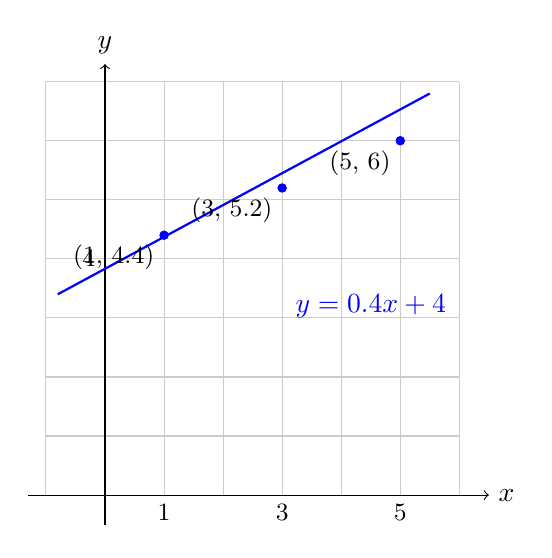
\begin{tikzpicture}[scale=0.75]
\draw[gray!40, step=1] (-1,0) grid (6,7);
\draw[->] (-1.3,0) -- (6.5,0) node[right] {$x$};
\draw[->] (0,-0.5) -- (0,7.3) node[above] {$y$};
\draw[blue, thick] (-0.8,3.4) -- (5.5,6.8);
\filldraw[blue] (1,4.4) circle (2pt) node[below left, black] {\small $(1,\,4.4)$};
\filldraw[blue] (3,5.2) circle (2pt) node[below left, black] {\small $(3,\,5.2)$};
\filldraw[blue] (5,6) circle (2pt) node[below left, black] {\small $(5,\,6)$};
\node[blue] at (4.5,3.2) {$y = 0.4x + 4$};
\node[below] at (1,0) {\small $1$};
\node[below] at (3,0) {\small $3$};
\node[below] at (5,0) {\small $5$};
\node[left] at (0,4) {\small $4$};
\end{tikzpicture}
\end{center}

上面这张图画的是直线 $y = 0.4x + 4$。为什么它的轨迹恰好是一条直线？看规则本身：$x$ 每增加 1，$y$ 就增加 0.4；$x$ 每增加 5，$y$ 就增加 2。增加的步伐永远一样大——匀速变化的轨迹不会拐弯，只能是直线。所有形如 $y = kx + b$（$k$、$b$ 是固定的数，$k \neq 0$）的函数都叫\textbf{一次函数}（或线性函数），它们的图像都是直线。

换一个规则试试：$y = x^2$。描几个点：

\begin{center}
\begin{tabular}{cccccccc}
\toprule
$x$ & $-3$ & $-2$ & $-1$ & $0$ & $1$ & $2$ & $3$ \\
\midrule
$y$ & $9$ & $4$ & $1$ & $0$ & $1$ & $4$ & $9$ \\
\bottomrule
\end{tabular}
\end{center}

注意表格里的对称：$(-2, 4)$ 和 $(2, 4)$ 一样高。把这些点连起来（为了让图能塞进书页，我们画它的缩小版 $y = \dfrac{1}{2}x^2 - 4$）：

\begin{center}
\begin{tikzpicture}[scale=0.75]
\draw[gray!40, step=1] (-4,-4) grid (4,4);
\draw[->] (-4.5,0) -- (4.5,0) node[right] {$x$};
\draw[->] (0,-4.5) -- (0,4.5) node[above] {$y$};
\draw[blue, thick] plot[smooth] coordinates {(-4,4) (-3,0.5) (-2,-2) (-1,-3.5) (0,-4) (1,-3.5) (2,-2) (3,0.5) (4,4)};
\filldraw[red] (0,-4) circle (2.2pt) node[below right, black] {\small 顶点 $(0,-4)$};
\draw[dashed, gray] (0,-4.5) -- (0,4.5);
\node[blue] at (2.9,-3.4) {$y = \frac{1}{2}x^2 - 4$};
\end{tikzpicture}
\end{center}

这条曲线叫\textbf{抛物线}。它不是直线的理由从表格里就能看出：$x$ 从 0 走到 1，$y$ 只挪动了一点；$x$ 从 2 走到 3，$y$ 却蹿了一大截。变化的步伐越来越快，轨迹当然要弯。抛向空中的皮球、喷泉里射出的水柱，走的都是这条曲线——这就是为什么你总觉得抛物线眼熟。

还有一种关系值得认识：\textbf{反比例}。班级凑 300 元包车去郊游，人均车费取决于去的人数 $x$：$y = \dfrac{300}{x}$。去 10 人，人均 30 元；去 30 人，人均 10 元；去 60 人，人均 5 元。人越多越便宜，但便宜的速度在放慢——从 10 人到 20 人，人均骤降 15 元；从 50 人到 60 人，只降了 1 元。它的图像是一条越来越贴近坐标轴、却永远碰不到轴的曲线（叫双曲线的一支）。路程固定时的速度与时间、矩形面积固定时的长与宽，都是反比例关系。

直线、抛物线、双曲线——三种轨迹，三种脾气。直线匀速，抛物线加速，双曲线先急后缓。你可能会问：既然规则都知道了，为什么还要画图？因为眼睛和大脑处理“形”的速度远快于处理“数”：一条曲线是升是降、是陡是缓、有没有最高点和最低点，扫一眼就明白，而这些信息埋在式子里要费一番功夫才能挖出来。图像是给规则做的一次“可视化体检”。

\section{斜率与截距：读懂函数的性格}

拿到一条直线的方程 $y = kx + b$，两个数字 $k$ 和 $b$ 各自管什么？

先看 $b$。当 $x = 0$ 时 $y = b$，所以 $b$ 是直线与 $y$ 轴交点的高度，叫\textbf{截距}。在出租车例子里，截距像“起步价”——还没开始按里程计价，账单上已经有的那部分。

再看 $k$。$x$ 每增加 1，$y$ 就增加 $k$，所以 $k$ 衡量这条直线的\textbf{陡峭程度}，叫\textbf{斜率}。斜率为正，直线从左往右爬坡；斜率为负，直线走下坡路；斜率的绝对值越大，坡越陡。

\begin{shuyu}{斜率}
\textbf{直观解释}：直线的“坡度”——水平方向每走 1 个单位，竖直方向上升多少。

\textbf{正式定义}：直线上任取两点 $(x_1, y_1)$ 和 $(x_2, y_2)$（$x_1 \neq x_2$），斜率
\[
k = \frac{y_2 - y_1}{x_2 - x_1}.
\]

\textbf{一个例子}：直线过 $(1, 4)$ 和 $(5, 12)$，斜率 $k = \dfrac{12 - 4}{5 - 1} = 2$，即每向右走 1，上升 2。
\end{shuyu}

斜率定义的下面藏着一个重要事实：这个比值和你选哪两个点\textbf{无关}。这并不平凡——为什么换两个点算出来的坡度一样？因为一次函数的变化是匀速的：$y_2 - y_1 = kx_2 + b - (kx_1 + b) = k(x_2 - x_1)$，一除恰好是 $k$，$b$ 被抵消了。反过来说，如果某个函数的“斜率”随位置变化，它的图像就一定不是直线——抛物线在山脚平缓、在半山腰陡峭，正是这个原因。

斜率还有个更响亮的名字：\textbf{变化率}。里程—车费直线的斜率是 2，意思是“每公里 2 元”；时间—路程直线的斜率是速度；时间—存款直线的斜率是存钱速度。读懂斜率，就读懂了“这个世界变化得有多快”。

斜率还带着单位，这一点常被忽略却极其有用。车费对里程的斜率单位是“元每公里”，路程对时间的斜率单位是“米每秒”——单位本身就告诉你这个变化率在度量什么。负斜率同样有意义：登山时海拔对时间的斜率是正的，下山时是负的；发烧时体温的斜率为正，退烧时为负。一条直线斜率的正负，讲的就是“这个量在涨还是在跌”。

\begin{fanli}
“$y$ 随着 $x$ 的增大而增大，所以 $y$ 和 $x$ 成正比例。”——错。反例：$y = x + 1$。$x$ 从 1 变到 2，$y$ 从 2 变到 3，确实在增大；但 $y$ 和 $x$ 的比值一会儿是 2、一会儿是 1.5，并不固定，$x = 0$ 时 $y$ 也不是 0。正比例要求图像是过原点的直线，即 $b = 0$。另一个相似的陷阱：“图像在上升，所以它是直线”——抛物线 $y = x^2$ 在 $x > 0$ 时也一直上升，可它分明是弯的。上升只说方向，不说形状。
\end{fanli}

反比例函数 $y = \dfrac{300}{x}$ 则展示了另一种性格：它没有一个统一的“斜率”，离原点近的地方陡得吓人，远处几乎平躺。变化率本身在变化——承认这一点，是人类数学史上的一次深呼吸，我们将在第 10 章正式面对它。

\section{换一个视角：图像替方程说话}

学会了看图像，我们回头看方程，眼光会完全不同。

方程 $2x + 5 = 21$ 是在问：直线 $y = 2x + 5$ 在高度 21 处的横坐标是多少？方程组
\[
\begin{cases}
y = 2x + 5,\\
y = -x + 23
\end{cases}
\]
是在问：这两条直线在哪里相交？画出来你会发现，两条不平行的直线恰好交于一点——这正是二元一次方程组通常有唯一解的几何原因。而 $x^2 - 10x + 24 = 0$ 是在问：抛物线 $y = x^2 - 10x + 24$ 在哪里贴着地面（与 $x$ 轴相交）？判别式为正，抛物线穿过地面两次；判别式为零，它刚好碰到地面就弹起来；判别式为负，它整个悬在半空——“没有实数解”在图像上就是“根本没碰着”。

\begin{lianjie}
第 1 章里，字母把一个个算术题压缩成代数式；这一章，图像又把代数式翻译回“形”。方程、函数、图像是同一件东西的三种语言：方程是审问（找出特定的 $x$），函数是全景（描述整个对应），图像是地图（把全景画给你看）。第 4 章我们会把这套翻译系统彻底打通，让几何图形直接变成代数方程。至于图像上的点、线、角到底凭什么可信——凭什么“看起来相交”就是真的相交——那是第 3 章要用证明来回答的问题。
\end{lianjie}

这种“换语言”的本事有实实在在的力量。面对一堆数据——比如过去一年每月的电费——直接看数字很难有感觉；描成图像，趋势、异常、周期全都跳出来。天气预报的温度曲线、股票软件的起起伏伏、体测报告里的生长曲线，背后都是同一句话：规则留下轨迹，轨迹泄露规则。

反方向同样行得通：把一个几何问题翻译成方程。公园喷泉的水柱是一条抛物线，设计师想让水柱在 4 米外落回水池、最高点 2 米——这些“形状上的要求”可以变成几个方程，解出来就得到喷口的精确参数。形状提要求，方程给答案，这是工程师每天都在做的事。我们第 4 章会系统地练习这门翻译。

\begin{shiyan}
\textbf{实验一：画一条自己的抛物线。}在方格纸上描出 $y = x^2$ 的 9 个点（$x$ 取 $-4$ 到 $4$），用光滑的曲线连接。然后做两件事：（1）沿 $y$ 轴对折纸张，看看两边是否重合；（2）用尺子量一量曲线在 $(1,1)$ 附近和 $(3,9)$ 附近的“坡度”，感受斜率随位置变化。

\textbf{实验二：测一测生活的斜率。}找一个有阶梯的地方，量出某一级台阶的高度和深度（比如高 15 厘米、深 28 厘米），算出坡度 $15 \div 28 \approx 0.54$。再找一段无障碍坡道做同样的测量，比较两者。你刚刚做的事情，和工程师设计坡道、和数学家定义斜率，是同一回事。
\end{shiyan}

\begin{toolbox}
本章你获得的新工具：
\begin{itemize}
\item \textbf{列方程}：给未知数起名字，把条件翻译成等式；多个未知数就列方程组，用代入消元。
\item \textbf{配方法与求根公式}：对付一切一元二次方程的通用程序；判别式 $b^2 - 4ac$ 先报“有没有解”。
\item \textbf{函数记号 $f(x)$}：把“对应规则”当作一个可以研究、可以起名字的对象。
\item \textbf{图像}：描点连线，把规则变成看得见的轨迹；直线、抛物线、双曲线是三种最常见的轨迹。
\item \textbf{斜率与截距}：一次函数的两个“性格参数”，分别管陡峭程度和起始位置；斜率就是变化率。
\end{itemize}
\end{toolbox}

\begin{pandeng}
继续往前，这些词会在更高处等你：\textbf{增长率与导数}（第 10 章，抛物线上每一点的“瞬时斜率”怎么定义）；\textbf{函数的复合与反函数}（把两台机器串联起来，以及把一台机器倒着开）；\textbf{指数函数与对数函数}（增长速度本身在增长的关系，比如细菌和存款）；\textbf{不动点}（有没有一个输入，机器吐出的恰好是它自己）。再远一点，大学数学会把“函数”这个词推广到难以想象的范围——函数之间也可以谈“距离”，函数的全体也可以组成一个“空间”。
\end{pandeng}

\section*{思考题}

\textbf{观察题}
\begin{sikao}
\item 在同一张坐标纸上画出 $y = 2x + 5$ 和 $y = -x + 23$，找到交点，再解方程组。交点坐标和方程组的解有什么关系？为什么会这样？\emph{提示：交点同时躺在两条直线上，意味着它的坐标同时让两个规则成立。}
\item 观察 $y = \dfrac{12}{x}$ 的函数值：$x$ 从 1 变到 2 时 $y$ 变了多少？$x$ 从 6 变到 7 时呢？两个区间一样长，为什么 $y$ 的变化差这么多？\emph{提示：把具体的 $y$ 值都算出来，比较两次“变化量”而不是“变化率”。}
\end{sikao}

\textbf{证明题}
\begin{sikao}
\item 证明：若两个正数之和固定为 10，则它们的乘积不超过 25，且只有当两数都等于 5 时取到 25。\emph{提示：设一个数为 $x$，另一个为 $10 - x$，把乘积写成二次式并配方；也可以想想本章围菜园的例子。}
\item 证明：设 $f(x) = kx + b$ 且 $k > 0$。若 $x_1 < x_2$，则 $f(x_1) < f(x_2)$（这称为“单调递增”）。\emph{提示：计算 $f(x_2) - f(x_1)$，利用 $x_2 - x_1 > 0$ 和 $k > 0$ 判断符号。}
\end{sikao}

\textbf{挑战题}
\begin{sikao}
\item 设 $x_1$、$x_2$ 是方程 $ax^2 + bx + c = 0$ 的两个解。不求出它们，直接证明 $x_1 + x_2 = -\dfrac{b}{a}$，$x_1 x_2 = \dfrac{c}{a}$。\emph{提示：把求根公式里的两个解原样相加、相乘，注意 $\sqrt{\phantom{a}}$ 会怎样消失；第 5 章会给这组关系一个专门的名字。}
\item 某城市的出租车计价规则是：3 公里以内 11 元，3 到 10 公里每公里 2 元，超过 10 公里的部分每公里 3 元。写出车费 $y$ 关于里程 $x$ 的分段表达式并画出图像。这台“机器”是函数吗？它的图像在 $x = 3$ 和 $x = 10$ 处发生了什么？\emph{提示：检查每个输入是否只有一个输出；图像不会断，但“坡度”会突然改变——这种点以后会有专门的名字。}
\end{sikao}

\section*{通往下一章的门}

这一章我们养成了一个习惯：凡是关系，就画成图像；凡是方程，就看成交点。图像成了我们最信任的眼睛。

但请你仔细回想一件小事：画抛物线的时候，你描了 9 个点，然后“用光滑的曲线连接”。凭什么？你只是看着那 9 个点大致在一条弯弯的轨道上，就顺手把它们连了起来。也许曲线在两个点之间偷偷拐了个你没看见的弯？也许你画的两条直线“看起来交在 $(6, 17)$”，量一量却是 $(5.98, 17.03)$？眼睛和尺子能帮我们发现线索，却永远不能替我们做担保——这正是数学里“测量”和“证明”的分界线。

下一章，我们回到比函数更古老的数学：点、线、角、三角形和圆。我们会看到，古希腊人如何从画不出一条“完美直线”的困境出发，建立起人类历史上第一座证明的大厦；也会看到同一个结论——比如那个关于直角三角形三边的著名定理——为什么值得用十几种不同的方式各证明一遍。图像让我们看见答案，证明让我们确信答案。现在，去认识第二样东西。
